\documentclass{standalone}
\usepackage{fontspec}
\setsansfont{DejaVuSans.ttf}[Path=./,Kerning=Off,Ligatures={TeXOff,NoCommon}]
\usepackage{tikz}
\begin{document}
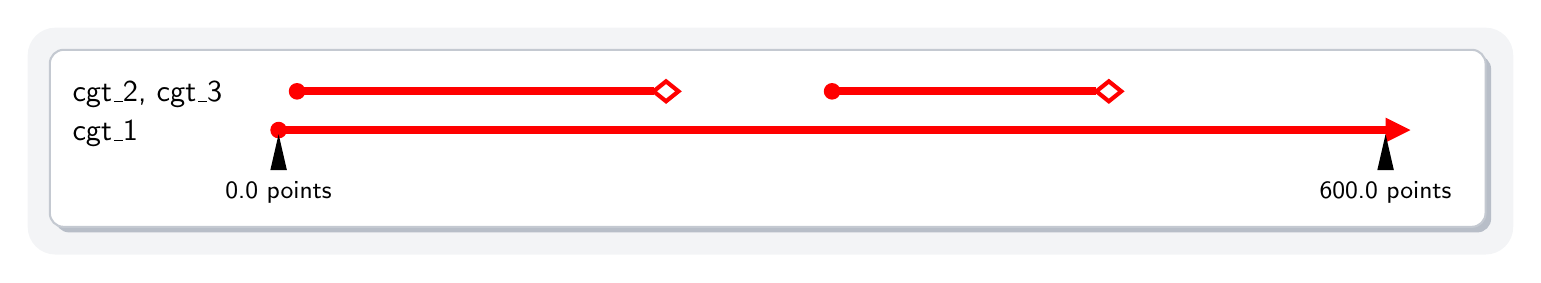
\begin{tikzpicture}[x=1pt,y=1pt,miter limit=4,font=\sffamily]
\definecolor{ts000000}{HTML}{000000}
\definecolor{tsB8BEC8}{HTML}{B8BEC8}
\definecolor{tsC4C9D1}{HTML}{C4C9D1}
\definecolor{tsF3F4F6}{HTML}{F3F4F6}
\definecolor{tsFF0000}{HTML}{FF0000}
\definecolor{tsFFFFFF}{HTML}{FFFFFF}
\begin{scope}[shift={(16,16)}]
\path[rounded corners=10pt,fill=tsF3F4F6] (0,0) rectangle (536.8105,81.9766);
\path[rounded corners=5pt,fill=tsB8BEC8] (10,8) rectangle (528.8105,71.9766);
\path[rounded corners=5pt,fill=tsFFFFFF,draw=tsC4C9D1,line width=0.75pt] (8,10) rectangle (526.8105,73.9766);
\path[draw=tsFF0000,line width=3pt] (90.6768,44.9766) -- (490.6768,44.9766);
\path[fill=tsFF0000] (90.6768,44.9766) circle[radius=3];
\path[fill=tsFF0000] (499.6768,44.9766) -- (490.6768,49.4766) -- (490.6768,40.4766) -- cycle;
\path[draw=tsFF0000,line width=3pt] (97.3434,58.9766) -- (226.1768,58.9766);
\path[fill=tsFF0000] (97.3434,58.9766) circle[radius=3];
\path[draw=tsFF0000,line width=1.5pt] (226.1768,58.9766) -- (230.6768,62.5766) -- (235.1768,58.9766) -- (230.6768,55.3766) -- cycle;
\path[draw=tsFF0000,line width=3pt] (290.6768,58.9766) -- (386.1768,58.9766);
\path[fill=tsFF0000] (290.6768,58.9766) circle[radius=3];
\path[draw=tsFF0000,line width=1.5pt] (386.1768,58.9766) -- (390.6768,62.5766) -- (395.1768,58.9766) -- (390.6768,55.3766) -- cycle;
\path[fill=ts000000] (90.6768,43.4766) -- (87.6768,30.4766) -- (93.6768,30.4766) -- cycle;
\path[fill=ts000000] (490.6768,43.4766) -- (487.6768,30.4766) -- (493.6768,30.4766) -- cycle;
\node[anchor=base west,inner sep=0,font=\sffamily\fontsize{11}{12.8047}\selectfont,text=ts000000] at (16,55.1685) {cgt\_2, cgt\_3};
\node[anchor=base west,inner sep=0,font=\sffamily\fontsize{11}{12.8047}\selectfont,text=ts000000] at (16,41.1685) {cgt\_1};
\node[anchor=base,inner sep=0,font=\sffamily\fontsize{9}{10.4766}\selectfont,text=ts000000] at (90.6768,20.1226) {0.0 points};
\node[anchor=base,inner sep=0,font=\sffamily\fontsize{9}{10.4766}\selectfont,text=ts000000] at (490.6768,20.1226) {600.0 points};
\end{scope}
\end{tikzpicture}
\end{document}
